\subsection{Condicionalidad: cGAN}
A diferencia de las tradicionales, las Redes Generativas Adversarias Condicionales (cGAN) permiten generar imágenes a partir de una condición explícita, como un vector de características derivado de una descripción textual. Esta capacidad resultaba fundamental para los objetivos del proyecto, por lo que se planteó como un enfoque prometedor desde el inicio.

\subsubsection{Librerías y Herramientas}
La implementación de la cGAN se llevó a cabo empleando herramientas ya utilizadas en la fase anterior con GAN básicas, como Keras y TensorFlow, por su robustez y facilidad de desarrollo. Además, se utilizaron NumPy y Matplotlib para el preprocesamiento de datos y la visualización de resultados, respectivamente. El dataset elegido fue COCO (Common Objects in Context), que destaca por incluir una gran variedad de imágenes, cada una acompañada por cinco descripciones textuales detalladas. Esto lo hace ideal para experimentar con modelos de generación condicionada por texto.

\subsubsection{Procesamiento de Texto}
Para representar las descripciones textuales de entrada, se probaron distintos enfoques. Inicialmente se utilizó \textit{one-hot encoding}, por su simplicidad de implementación, aunque se descartó rápidamente debido a su alta dimensionalidad y su incapacidad para capturar relaciones semánticas entre palabras.

Posteriormente, se probó Word2Vec, que transforma palabras en vectores de características en un espacio semántico. Esta técnica mejoró la representación textual, pero mostró limitaciones al no capturar adecuadamente la estructura de las frases ni las relaciones entre los objetos.

Finalmente, se optó por trabajar directamente con las descripciones originales del dataset COCO, que ya estaban preprocesadas y estructuradas. Estas descripciones fueron tokenizadas y limpiadas para eliminar ruido textual. Se utilizaron embeddings preentrenados como los de CLIP, que transforman las frases en vectores latentes significativos para la generación de imágenes. Esta solución resultó más robusta, computacionalmente eficiente y adecuada para preservar la semántica de las descripciones complejas.

\subsubsection{Pruebas preliminares con MNIST}
Antes de abordar un dataset complejo como COCO, se realizó una prueba de concepto utilizando el conjunto de datos MNIST. Este dataset contiene imágenes de dígitos del 0 al 9, por lo que era ideal para comprobar la capacidad de la cGAN para generar imágenes condicionadas.

Se codificaron los dígitos como vectores one-hot y se concatenaron con el ruido aleatorio que se proporciona al generador. El modelo se entrenó durante 50 épocas con una tasa de aprendizaje de 0.0002 y un tamaño de batch de 64. Al principio, las imágenes eran borrosas, pero al finalizar el entrenamiento, la cGAN era capaz de generar dígitos nítidos y variados, respetando la condición de entrada. Este comportamiento puede observarse en la Figura \ref{fig:numeros_0-9}, que muestra los dígitos generados al final del proceso. Esto confirmó la viabilidad del enfoque condicional.

\begin{figure}[H]
\centering
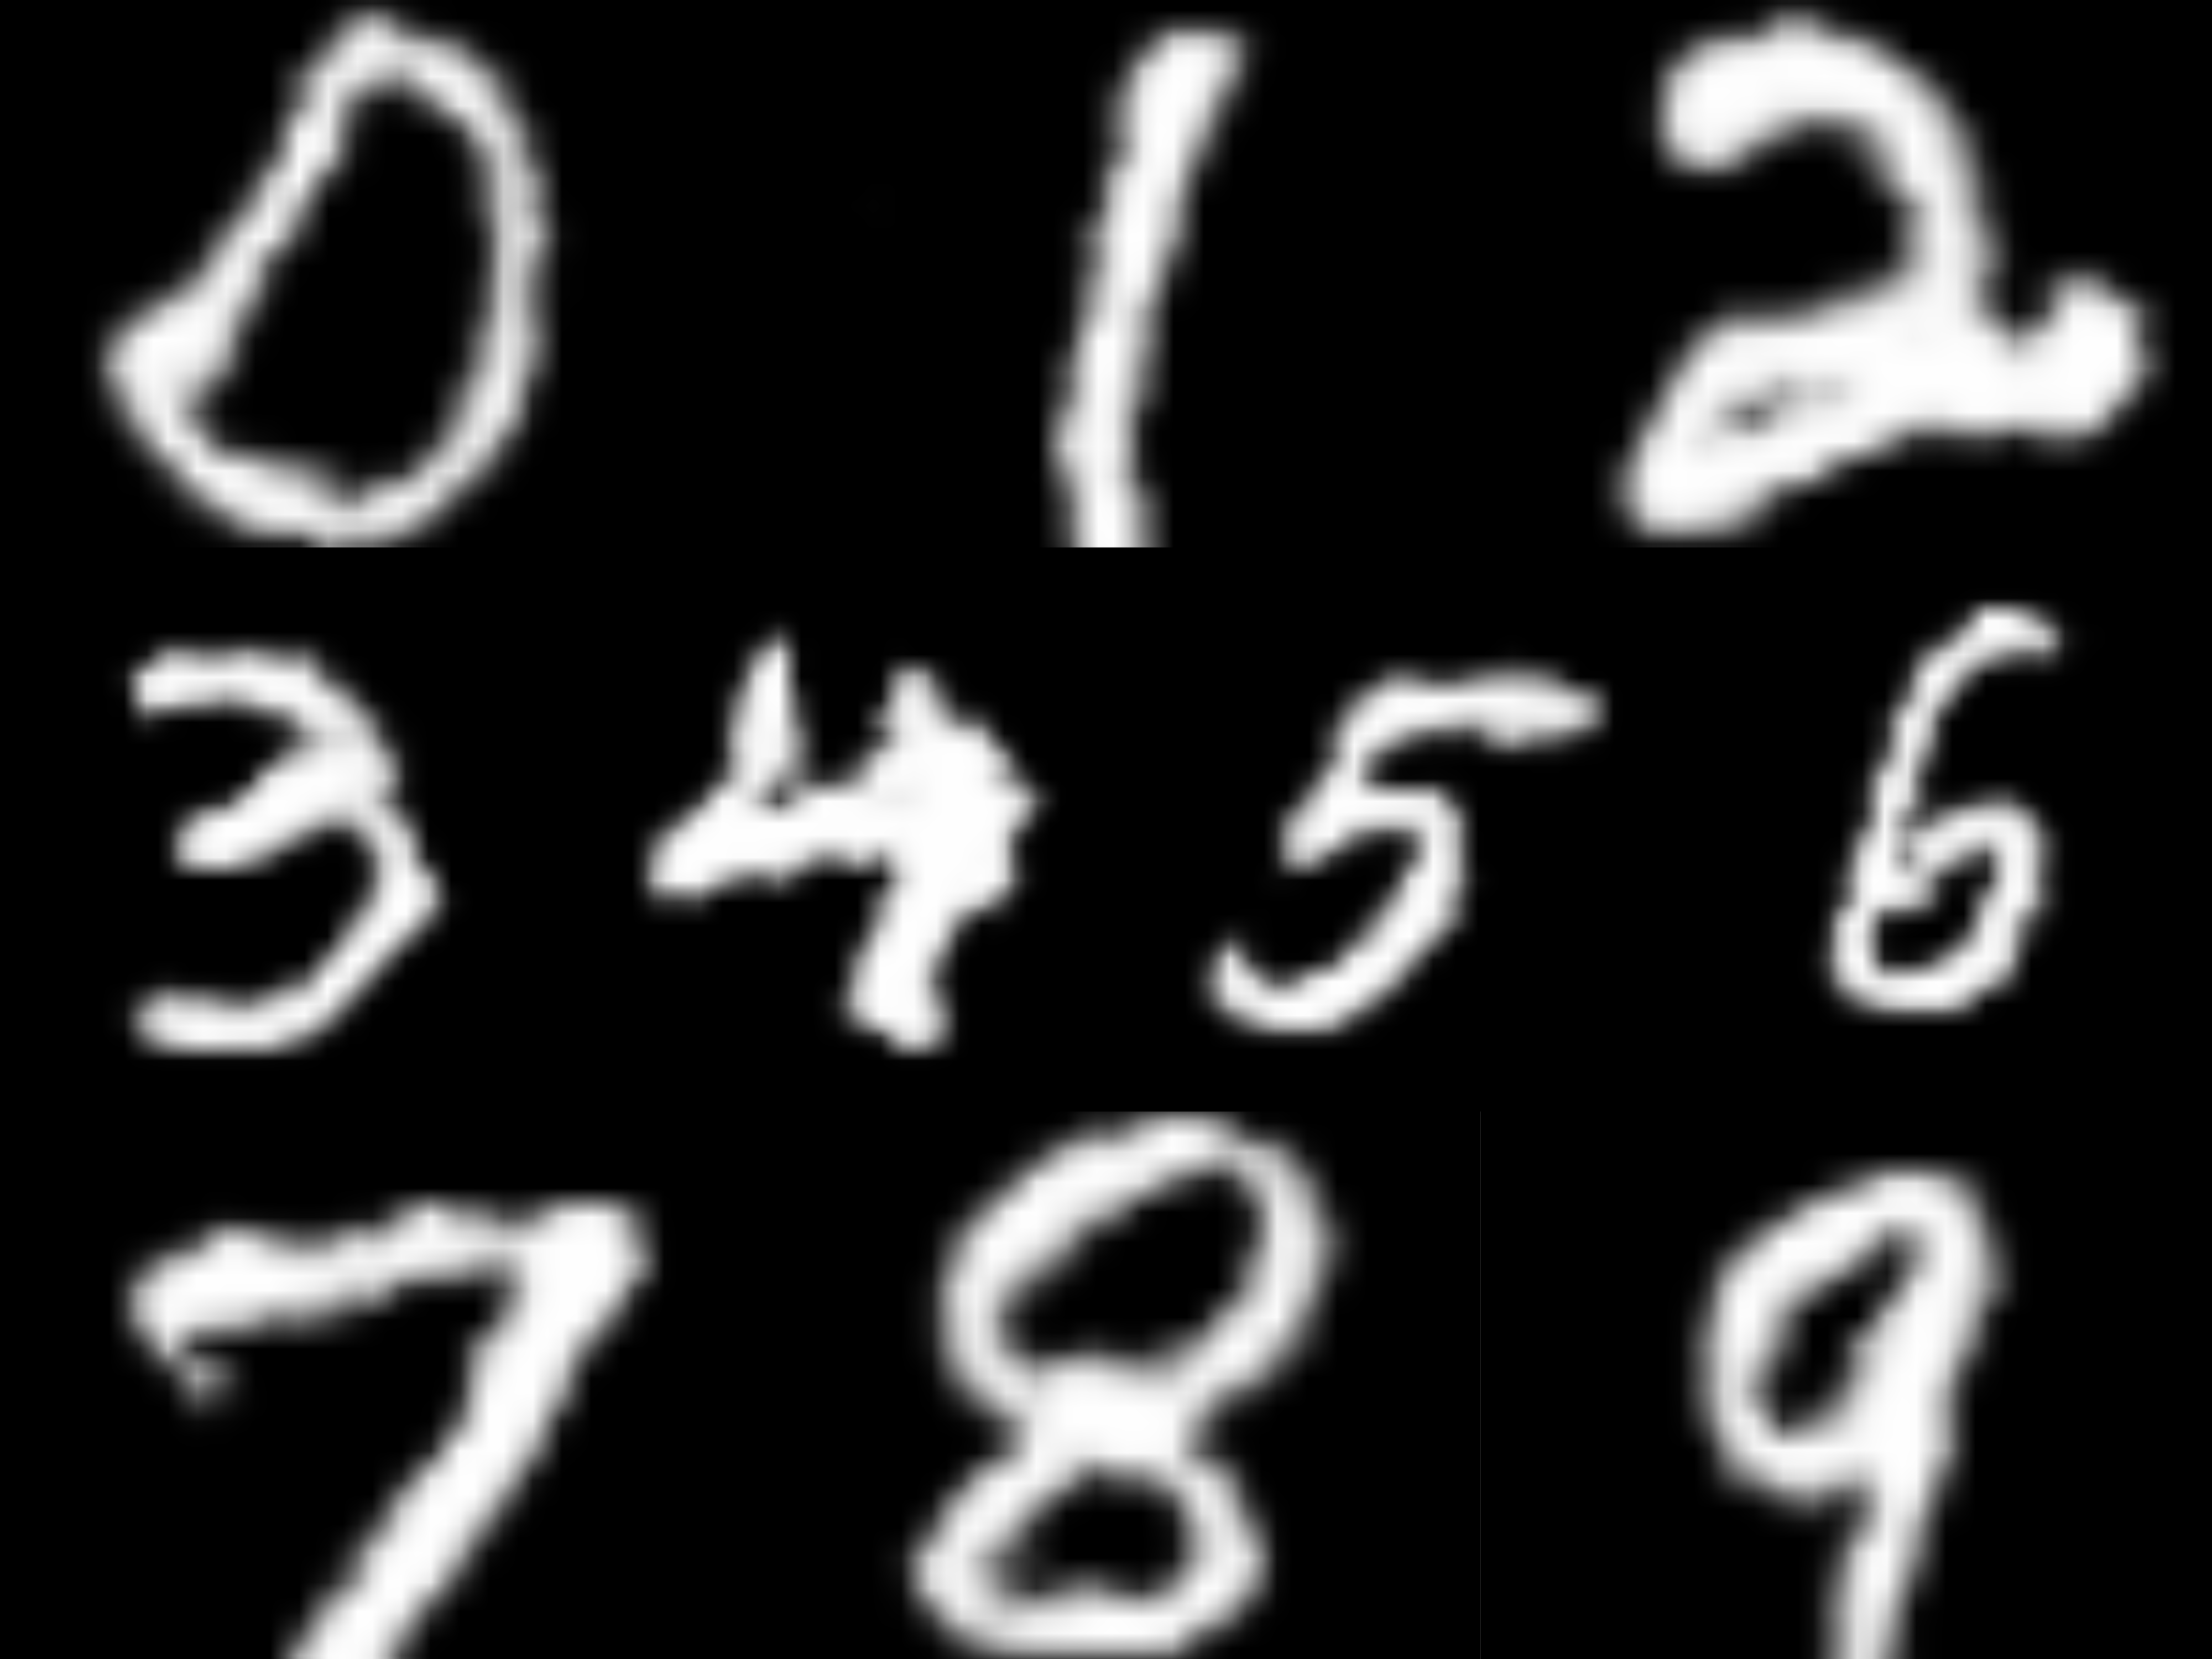
\includegraphics[width=0.4\textwidth]{mnist/resultado_0-9}
\caption{Imágenes generadas con el modelo entrenado con MNIST}
\label{fig:numeros_0-9}
\end{figure}

\subsubsection{Datasets}
El modelo fue entrenado con el dataset COCO en dos variantes. Por un lado, se utilizó el conjunto completo, que ofrece una gran variedad de escenarios y contextos, lo que mejora la generalización del modelo. Sin embargo, su alto requerimiento computacional exigía un entorno potente y tiempos prolongados de entrenamiento.

Por otro lado, se trabajó con subconjuntos aleatorios del dataset, lo que permitía experimentar con mayor agilidad y requerimientos más modestos de memoria. Si bien esto limitaba la generalización, resultó útil para afinar hiperparámetros y realizar pruebas rápidas.

\subsubsection{Pruebas y resultados}
La arquitectura de la cGAN fue adaptada para trabajar con entrada condicionada, lo que implicó modificaciones específicas tanto en el generador como en el discriminador. El generador fue diseñado para recibir un vector de ruido aleatorio concatenado con un vector de características textuales, representando la descripción de la imagen deseada. Este vector conjunto alimentaba una red de capas transpuestas convolucionales que generaban una imagen de salida. Por su parte, el discriminador fue ajustado para aceptar como entrada tanto la imagen generada como la descripción textual correspondiente, evaluando si la imagen no solo era realista, sino también coherente con el texto proporcionado.

Durante el proceso de entrenamiento, se llevaron a cabo múltiples fases de pruebas, con ajustes progresivos que permitieron estudiar el comportamiento del modelo ante diferentes configuraciones:

\begin{itemize}
\item \textbf{Primera etapa:} Se utilizó una tasa de aprendizaje de 0.0002 y se mantuvo una arquitectura básica en el generador y el discriminador. En esta configuración, el modelo logró generar imágenes con formas básicas y contornos generales, pero sin mucho detalle. Las imágenes eran a menudo borrosas y poco realistas, especialmente cuando las descripciones textuales eran más complejas o contenían múltiples objetos.

\item \textbf{Segunda etapa:} Se redujo la tasa de aprendizaje a 0.0001, buscando una mayor estabilidad en el proceso de entrenamiento. Este ajuste permitió al modelo generar imágenes con mayor nitidez en los bordes y una ligera mejora en la estructura general de los objetos. No obstante, aún persistía cierta borrosidad, especialmente cuando el texto incluía relaciones espaciales o adjetivos calificativos que requerían una interpretación semántica más profunda.

\item \textbf{Tercera etapa:} Se realizaron modificaciones más profundas en la arquitectura, incrementando la profundidad de las redes LSTM utilizadas para procesar el texto y añadiendo capas convolucionales adicionales al generador. Estos cambios permitieron al modelo capturar mejor los detalles visuales descritos en las anotaciones textuales. Las imágenes generadas mostraban una mayor fidelidad a las descripciones, especialmente en contextos sencillos o escenas con un número limitado de elementos. Sin embargo, cuando las descripciones eran más complejas, que incluían múltiples objetos en relación o elementos abstractos, el modelo aún presentaba dificultades para generar imágenes coherentes.

\end{itemize}

En conjunto, estas pruebas demostraron que la arquitectura de la cGAN, con un ajuste adecuado de hiperparámetros y arquitectura, era capaz de generar imágenes razonablemente alineadas con descripciones textuales simples, aunque todavía mostraba limitaciones en cuanto a la representación semántica profunda y la calidad visual en escenarios complejos.


\subsubsection{Pruebas con diferentes números de épocas}
Se compararon dos enfoques de entrenamiento para evaluar cuál ofrecía mejores resultados bajo distintas condiciones de entrenamiento y disponibilidad de recursos computacionales:

\begin{itemize}
\item \textbf{Entrenamiento en múltiples fases cortas (menos épocas)}: Este enfoque consistía en entrenar el modelo con un número reducido de épocas, interrumpir el proceso, analizar los resultados obtenidos y realizar ajustes en los hiperparámetros o en la arquitectura antes de retomar el entrenamiento. Su principal ventaja radica en la velocidad de iteración, permitiendo una retroalimentación rápida sobre el comportamiento del modelo. Esto resultó útil especialmente en las primeras fases de desarrollo, donde se requería probar distintas combinaciones de parámetros y realizar modificaciones frecuentes. Sin embargo, se observó que este tipo de entrenamiento limitaba el potencial de aprendizaje del modelo, ya que no se alcanzaban suficientes ciclos de optimización para capturar patrones más complejos del conjunto de datos. Además, las mejoras en la calidad de las imágenes generadas tendían a estancarse tras unas pocas épocas.

\item \textbf{Entrenamiento continuo con muchas épocas}: En contraste, este enfoque implicaba ejecutar el entrenamiento de manera prolongada, permitiendo que el modelo tuviese tiempo suficiente para ajustar de forma más precisa los pesos de sus redes. Esta estrategia fue especialmente efectiva una vez se contaba con una configuración inicial bien afinada, ya que permitía que el modelo convergiera hacia una solución más estable y generara imágenes de mayor calidad. Las imágenes resultantes presentaban mayor nivel de detalle y coherencia con las descripciones textuales. No obstante, este método también conllevaba riesgos, como el sobreajuste, especialmente si los hiperparámetros no estaban correctamente definidos. Además, al requerir mayor tiempo y recursos computacionales, su ejecución resultaba menos viable en fases iniciales de desarrollo o cuando se contaba con recursos limitados.

\end{itemize}

Ambos métodos ofrecieron ventajas complementarias. El entrenamiento en fases cortas fue ideal para la exploración rápida y la experimentación con diferentes configuraciones, mientras que el entrenamiento extendido resultó más adecuado en etapas finales, cuando se buscaba optimizar la calidad del modelo ya ajustado. En el contexto del proyecto, se utilizó una combinación de ambos enfoques: primero se realizaron múltiples entrenamientos breves para afinar la arquitectura y los hiperparámetros, y posteriormente se aplicó un entrenamiento largo con la configuración seleccionada para maximizar el rendimiento final del modelo. Las diferencias entre ambos enfoques, así como sus principales ventajas y desventajas, se resumen en la Tabla~\ref{tab:comparacion_entrenamiento}.


\begin{table}[H]
\centering
\renewcommand{\arraystretch}{1.5}
\begin{tabular}{p{5cm}p{5cm}p{5cm}}
\rowcolor{gray!30}
\textbf{Aspecto} & \textbf{Entrenar varias veces con menos épocas} & \textbf{Entrenar una sola vez con más épocas} \\
\rowcolor{gray!10}
\textbf{Velocidad de iteración} & Alta: permite detectar problemas y ajustar configuraciones rápidamente & Baja: requiere más tiempo para identificar problemas o ajustar parámetros \\
\addlinespace
\textbf{Potencial de aprendizaje} & Limitado, ya que el modelo no alcanza su máximo potencial & Alto, permite que el modelo ajuste mejor los pesos y logre mayor detalle \\
\rowcolor{gray!10}
\textbf{Riesgo de sobreajuste} & Bajo, debido a la menor cantidad de épocas & Alto, especialmente si la configuración inicial no es óptima \\
\addlinespace
\textbf{Calidad de las imágenes} & Adecuada para configuraciones iniciales, pero se estanca en calidad final & Mejor calidad, con imágenes más detalladas y coherentes \\
\rowcolor{gray!10}
\textbf{Flexibilidad en ajustes} & Alta: permite ajustar configuraciones con mayor frecuencia & Baja: los errores solo se detectan al final del proceso \\
\addlinespace
\textbf{Uso de recursos} & Menor uso de recursos en cada iteración & Mayor uso de recursos debido a entrenamientos más largos \\
\rowcolor{gray!10}
\textbf{Idoneidad} & Ideal para experimentación y ajustes rápidos & Adecuado para optimización final con configuraciones ajustadas \\
\end{tabular}
\caption{Comparativa entre entrenar con menos épocas y entrenar con más épocas}
\label{tab:comparacion_entrenamiento}
\end{table}

\subsubsection{Visualización de pérdidas}
Las curvas de pérdida registradas durante el entrenamiento muestran que el discriminador aprende rápidamente en las primeras épocas, con una pérdida que disminuye rápidamente. En contraste, el generador progresa más lentamente, con una pérdida que decrece gradualmente. Este comportamiento es común en las cGAN, y si no se controla, puede llevar a un desequilibrio en el entrenamiento. En este caso, el discriminador tendía a dominar, lo que podría afectar negativamente la calidad de las imágenes generadas.

\begin{figure}[H]
\centering
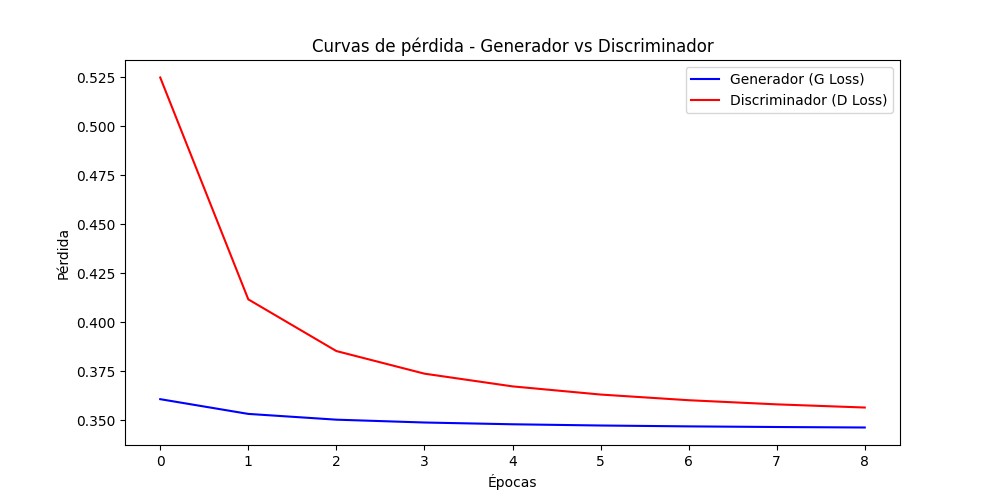
\includegraphics[width=0.7\textwidth]{perdidas}
\caption{Curva de pérdidas durante el entrenamiento de la cGAN}
\label{fig:loss_curve_cgan}
\end{figure}

\subsubsection{Conclusión}
La cGAN permitió integrar las descripciones textuales en el proceso de generación de imágenes, obteniendo mejores resultados que con la GAN básica. Sin embargo, el modelo mostró dificultades para representar con nitidez descripciones complejas. Esto motivó la exploración de modelos más sofisticados como la AttnGAN, que incorpora mecanismos de atención para mejorar la correspondencia entre texto e imagen.
